\documentclass{juliacon}
\usepackage{amsmath}
\usepackage{float}
\setcounter{page}{1}

\begin{document}

\title{DisjunctiveProgramming.jl: Generalized Disjunctive Programming Models and Algorithms for JuMP}
\author{
  \large Hector D. Perez*, Shivank Joshi, Ignacio E. Grossmann
  \\\normalsize Carnegie Mellon University, Pittsburgh, PA, USA  
  \\\normalsize	*hdperez@cmu.edu
}

\maketitle


\section*{ABSTRACT}
We present a Julia package, \textit{DisjunctiveProgramming.jl}, that extends the functionality in \textit{JuMP.jl} to allow modeling problems via logical propositions and disjunctive constraints \cite{dunning_huchette_lubin_2017}. Logical propositions are converted into algebraic expressions by converting the Boolean expressions to Conjunctive Normal Form and then to algebraic inequalities. The package allows the user to specify the technique to reformulate the disjunctions (Big-M or Hull reformulations) into mixed-integer constraints. This allows generating models that can be solved by the various MIP solvers supported by JuMP \cite{DunningHuchetteLubin2017}. The package supports reformulations for disjunctions containing linear, quadratic, and nonlinear constraints.

\section*{Keywords}
Julia, Optimization, Mathematical programming, \\ Generalized disjunctive programming

\section{Introduction}
The modeling of systems with discrete and continuous decisions is commonly done in algebraic form with mixed-integer programming (MIP) models. This is the standard approach for setting up problems that are linear or nonlinear in their continuous variables.
\vskip 6pt
A more systematic approach to modeling such systems is to use Generalized Disjunctive Programming (GDP) TODO (Chen \& Grossmann, 2019; Grossmann \& Trespalacios, 2013), which generalizes the Disjunctive Programming paradigm proposed by Balas \cite{balas_2018}. GDP enables the modeling of systems from a logic-based level of abstraction that captures the fundamental rules governing such systems via algebraic constraints and logic. This formulation is useful for expressing problems in an intuitive way that matches their logical structure, without needing to translate the logical statements into mathematical form. 
\vskip 6pt
The models obtained via GDP can then be reformulated into the pure algebraic form best suited for the application of interest. These models group related constraints into disjuncts to keep GDP models highly organized. It is also often possible to exploit the explicit logical structure of a GDP model to provide tighter relaxations than corresponding MIP models, which may improve convergence speed and robustness for solutions via advanced solution algorithms TODO (Chen \& Grossmann, 2019).
\vskip 6pt
There is currently high volume of ongoing research using GDP to formulate models for a variety of applications. Due to the combinatorial nature of system design problems, the GDP paradigm is commonly applied to the optimization of design synthesis for complex sequential processes and networks \cite{MATOVU2022107856, ZHOU202269}. Other work using the GDP approach is in the area of planning and optimal control for energy systems \cite{CHO2022841, kim2022generalized}. There is also ongoing research to further develop the generalized disjunctive programming approach, handling uncertainties in the chemical synthesis area \cite{CHEN2022107616}. These numerous applications of GDP illustrate the benefit of a robust package to abstract away some of the overhead associated with developing and testing GDP models to accelerate research.
\vskip 6pt
This paper provides background information on the GDP paradigm and a review of techniques for reformulating and solving models. It then presents the package DisjunctiveProgramming.jl as an extension to \verb|JuMP.jl| for creating models for optimization that follow this modeling paradigm. A case study demonstrates the use of the package for optimization over a chemical process superstructure.

\section{Generalized Disjunctive Programming}
The GDP form of modeling is an abstraction that uses both algebraic and logical constraints to capture the fundamental rules governing a system. The models obtained via GDP can then be reformulated into the mixed-integer algebraic form best suited for the application of interest. The two main reformulation strategies are the Big-M reformulation \cite{nemhauser_1999, TRESPALACIOS201598} and the Hull reformulation \cite{LEE20002125}, the latter of which yields tighter models at the expense of larger model sizes \cite{grossmann_lee_2003}. 
\vskip 6pt

\subsection{Formulation of Problem}
The notation for a general decision process with continuous and discrete variables written in the Mixed-Integer Nonlinear Programming (MINLP) problem is as follows:
\begin{align*}
    \min &f(x, y) \\
    \text{s.t.} \ &g(x, y) \leq 0 \\
    & h(x, y) = 0 \\
    & x \in X \subset \mathbb{R}^n \\
    & y \in Y \subset \mathbb{Z}^m
\end{align*}
In the above notation, x is the set of continuous variables, y is the set of discrete variables, and $f$ is the objective function to be minimized. $g$ and $h$ are functions representing the inequality and equality constraints on the problem, respectively \cite{chen_grossmann_2019}.
\vskip 6pt

The general notation for a disjunction in a GDP problem is
\begin{align*}
    \min \ &f(x, y) \\
    \text{s.t.} \ &g(x, y) \leq 0 \\
    &\bigvee_{i \in D_k}
    \begin{bmatrix}
        \Upsilon_{i,k} \\
        h_{i,k}(x, z) \leq 0
    \end{bmatrix}, \ \forall k \in K \\
    & \Omega(\Upsilon) = True \\
    & \Upsilon_{i,k} \in \{0, 1\} \\
    & x \in X \subset \mathbb{R}^n \\
    & y \in Y \subset \mathbb{Z}^m
\end{align*}
\vskip 6pt

Here, there are k disjunctions with i terms each, and constraint functions $h$, are applied only if the respective disjunct's term's indicator variable, $\Upsilon$, is denoted as being active \cite{chen_grossmann_2019}. The set of logical propositions, $\Omega$, describe logical relationships between the selections of indicator variables.
\vskip 6pt

In the case of a linear objective and set of constraints, the GDP model can be written as
\vskip 6pt
\begin{align*}
    \min \ & c^Tx \\
    \text{s.t.} \ &Ax \leq b \\
    &\bigvee_{i \in D_k}
    \begin{bmatrix}
        z_{i,k} \\
       B_{i,k}x \leq d_{i,k}
    \end{bmatrix}, \ k \in K \\
    & \Omega(z) = True \\
    & z_{i,k} \in \{0, 1\}
\end{align*}
\vskip 6pt

In this notation, $x$ groups discrete and continuous variables.
\vskip 6pt

\subsection{Linear GDP reformulation example}
The simplest example of a linear GDP system is given in \eqref{eq:ex} - \eqref{eq:y}, where $y_i$ is a Boolean indicator variable that enforces the constraints in the disjunct ($Ax \le b$ or $Cx \le d$) when $true$.
\vskip 6pt
\begin{equation}
    \label{eq:ex}
    \begin{bmatrix}
    y_1 \\ Ax \leq b
    \end{bmatrix}
    \lor
    \begin{bmatrix}
        y_2 \\ Cx \leq d
    \end{bmatrix}
\end{equation}
\begin{equation}
    \label{eq:x}
    0 \leq x \leq U
\end{equation}
\begin{equation}
    \label{eq:y}
    y_i \in \{true, false\} \quad \forall i\in \{1,2\}
\end{equation}
\vskip 6pt

For the purpose of visualization of the following reformulations of the feasible space, the simple example of a feasible solution space in \ref{fig:reform_figure} will be used without loss of generality.

\begin{figure}[H]
    \centering
    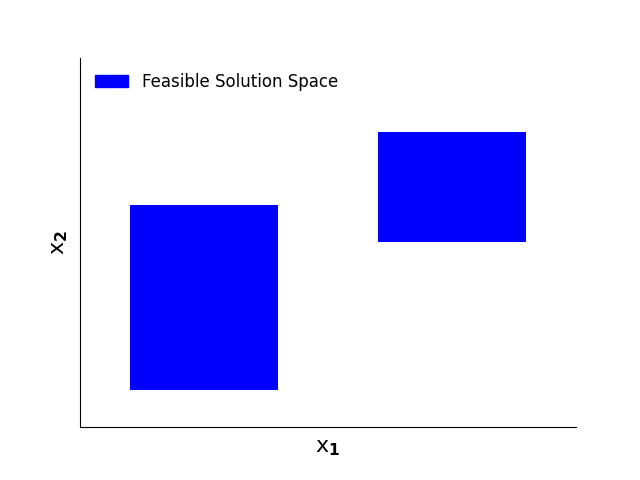
\includegraphics[scale=0.5]{solnspace.png}
    \caption{Feasible solution space for example disjunction}
    \label{fig:reform_figure}
\end{figure}
\vskip 6pt

 \subsubsection{Big-M Reformulation}
 The Big-M reformulation for this problem is given by \eqref{eq:x}, \eqref{eq:ex_bigm1} - \eqref{eq:ex_bigm4}.
 \vskip 6pt
 
\begin{equation}
    \label{eq:ex_bigm1}
    Ax \leq b + M \cdot (1 - y_1)
\end{equation}
\begin{equation}
    \label{eq:ex_bigm2}
    Cx \leq d + M \cdot (1 - y_2)
\end{equation}
\begin{equation}
    \label{eq:ex_bigm3}
    y_1 + y_2 = 1
\end{equation}
\begin{equation}
    \label{eq:ex_bigm4}
    y_i \in \{0,1\} \quad \forall i \in \{1,2\}
\end{equation}
\vskip 6pt

This reformulation can be visualized by the region encapsulated by the dashed line in \ref{fig:bigm}. Note that the relaxed region is not as tight as possible around the feasible solution space. The choice of large 'M' value determines the tightness of this relaxation, and the minimal value of 'M' for the optimal relaxation can be found through interval arithmetic.
\begin{figure}[h]
    \centering
    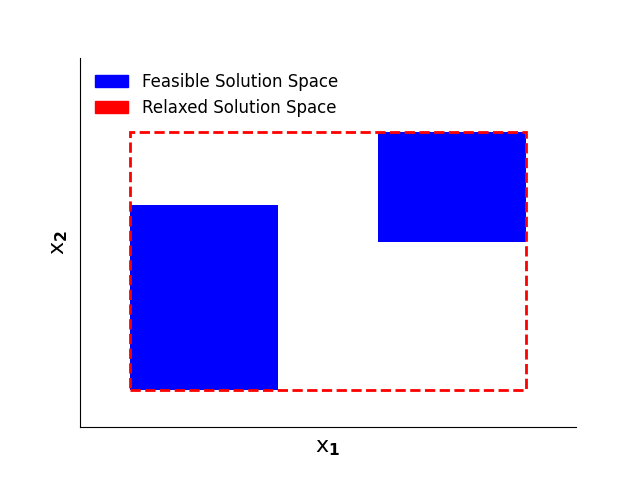
\includegraphics[scale=0.5]{bigm.png}
    \caption{Relaxed solution space using Big-M Reformulation}
    \label{fig:bigm}
\end{figure}
\vskip 6pt

\subsubsection{Convex Hull Reformulation}
The Hull reformulation is given by \eqref{eq:ex_bigm3} - \eqref{eq:ex_hull3}, which requires lifting the model to a higher-dimensional space. When projected to the original space, the continuous relaxation of the model is tighter than its Big-M equivalent (Grossmann \& Trespalacios, 2013).
\vskip 6pt
\begin{equation}
    \label{eq:ex_hull1}
    Ax_1 \leq by_1
\end{equation}
\begin{equation}
    \label{eq:ex_hull0}
    Cx_2 \leq dy_2
\end{equation}
\begin{equation}
    \label{eq:ex_hull2}
    x = x_1 + x_2
\end{equation}
\begin{equation}
    \label{eq:ex_hull3}
    0 \leq x_i \leq U y_i \quad \forall i \in \{1,2\}
\end{equation}
\vskip 6pt

This reformulation can be visualized by the region encapsulated by the dashed line in \ref{fig:chr}. Note that this reformulation provides a tighter relaxation than the Big-M reformulation. Also note that describing the geometry of this relaxation is more complex than the Big-M relaxation, and this increases the relative size of the model.
\vskip 6pt
\begin{figure}[H]
    \centering
    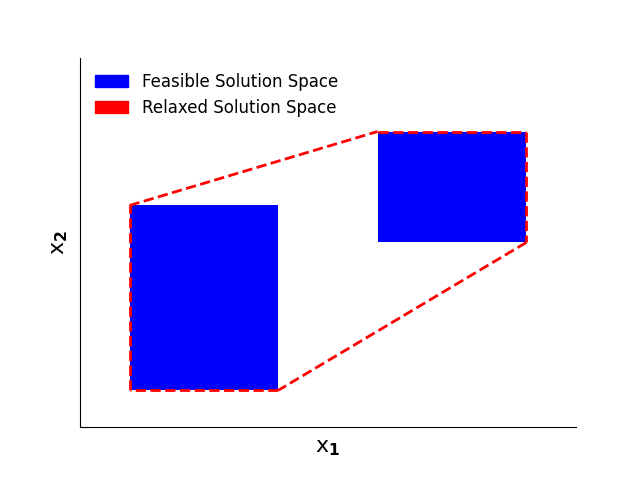
\includegraphics[scale=0.5]{chr.png}
    \caption{Relaxed solution space using Hull Reformulation}
    \label{fig:chr}
\end{figure}
\vskip 6pt


\subsection{Model Logical Constraint Reformulation}

\subsubsection{Propositional Logic}
The logical propositions within the set of decision selection relationships, $\Omega$, must be converted into conjunctive normal form (CNF) prior to solving a GDP model. This means that each phrase within the let of propositions must be formulated into a conjunction of disjunctions. This process can be accomplished by following the simplifying rules of propositional logic as follow:
\vskip 6pt

For boolean variables $A$, $B$, and $C$,
\begin{align*}
    A \leftrightarrow B & \cong (A \rightarrow B) \land (B \rightarrow A) \\
    A \rightarrow B & \cong \lnot A \lor B \\
    \lnot(A \lor B) & \cong \lnot A \land \lnot B \\
    \lnot(A \land B) & \cong \lnot A \lor \lnot B \\
    (A \land B) \lor C & \cong (A \lor C) \land (B \lor C)
\end{align*}
\vskip 6pt

More complex approaches to CNF conversion involve preserving phrase satisfiability rather than phrase equivalence, which prevents exponential size increase in phrases and yields logically consistent results. \cite{jackson_sheridan_2005}.
\vskip 6pt

\subsubsection{Constraint Programming}
The requirements for constraints within $\Omega$ are also reformulated as follows:
\vskip 6pt
\begin{align*}
    \text{exactly}(n, Y) & \rightarrow n = \sum_i Y_i \\
    \text{atleast}(n, Y) & \rightarrow n \leq \sum_i Y_i \\
    \text{atmost}(n, Y) & \rightarrow n \geq \sum_i Y_i
\end{align*}
\vskip 6pt
for $n$ boolean variables $Y$.
\vskip 6pt

\subsection{Solution Techniques}

\subsubsection{Disjunctive branch and bound}
The disjunctive branch and bound method closely mirrors the standard branch and bound approach for the solution of mixed-integer programming problems \cite{grossmann_lee_2003}. This algorithm iterates to converge to a solution by first solving a relaxed version of the problem and assigning a value, $\lambda$, to each term in each disjunction corresponding to how close the disjunct's constraints are to being satisfied. Then, the disjunct closest to being satisfied is fixed and each branch stemming from this problem is added to a queue. As long as there are problems on the queue, this algorithm iterates. If a solution is found, the problem is solved. If there is no solution found and the queue is empty, the problem is infeasible.
\vskip 6pt

\subsubsection{Logic-based outer approximation}
Logic-based outer approximation is another algorithm which mirrors a standard technique for solving mixed integer programming problems \cite{E.Grossmann2009}. This approach starts by identifying sub-problems of the GDP model to solve in order to encompass each set of disjunctions. Then, each subproblem is solved to find optimal solutions which serve as upper bounds. These solutions are used to locally linearize the objective and constraints of the original problem and solve the resulting problem to find a lower bound. If the lower and upper bound solutions have not converged, fix the boolean variables from the previous solution and solve this problem to find a potentially tighter upper bound solution. If the bounds have still not converged, repeat the process, linearizing the problem and resolving.
\vskip 6pt

\subsubsection{Hybrid cutting planes}
The cutting planes method is an algorithm for tightening the relaxed solution space of a problem reformulated with Big-M before solving it by adding additional constraints which remove parts of the relaxed space that are disjoint from the actual feasible solution space. These 'cuts' to the relaxed solution space are derived from the tighter, convex-hull relaxation for the problem. This algorithm provides a middle-ground for the tradeoff between the complexity and corresponding computational expense of the Convex Hull reformulation with the less tight Big-M reformulation. \cite{trespalacios_grossmann_2016}. 
\vskip 6pt


\section{DisjunctiveProgramming.jl}
\subsection{Features}


\subsection{Example}
To illustrate the syntax in \textit{DisjunctiveProgramming.jl} (Version 0.3.2), consider the simple superstructure optimization problem for the chemical process given in Figure \ref{fig:superstruct_opt_diagram}. The GDP model seeks to maximize the product flow ($F_7$), while discounting for reactor ($CR$) and separator ($CS$) installation costs as given in \eqref{eq:example_obj}, subject to the nested disjunction in \eqref{eq:example_gdp} and the global mass balances in \eqref{eq:example_global}
- \eqref{eq:example_global1}. The system variables are the flows on each stream $i$ ($F_i$) and the installation costs, with their respective bounds given in \eqref{eq:example_var1} - \eqref{eq:example_var3}. The fixed cost and process yield parameters are given by $\gamma$ and $\beta$, respectively.
\vskip 6pt

\begin{figure}[h]
    \centering
    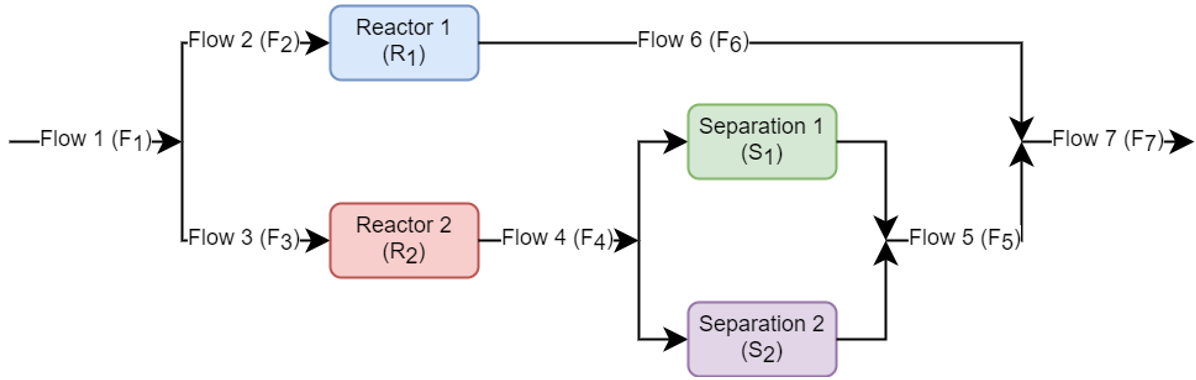
\includegraphics[scale=0.4]{juliacon pfd ss.png}
    \caption{Illustrative superstructure optimization problem}
    \label{fig:superstruct_opt_diagram}
\end{figure}
\begin{equation}
    \label{eq:example_obj}
    \max F_7 - CR - CS
\end{equation}
\begin{equation}
    \label{eq:example_gdp}
    \begin{bmatrix}
        Y_{R1} \\
        F_6 = \beta_{R1} F_2 \\
        F_3 = 0 \\
        F_4 = 0 \\
        F_5 = 0 \\
        C_R = \gamma_{R1} \\
        CS = 0
    \end{bmatrix} \lor
    \begin{bmatrix}
        Y_{R2} \\
        F_2 = 0 \\
        F_6 = 0 \\
        F_4 = \beta_{R2} F_3 \\
        C_R = \gamma_{R2} \\
        \begin{bmatrix}
            Y_{S1} \\
            F5 = \beta_{S1} F_4 \\
            C_S = \gamma_{S1}
        \end{bmatrix} \lor
        \begin{bmatrix}
            Y_{S2} \\
            F5 = \beta_{S2} F_4 \\
            C_S = \gamma_{S2}
        \end{bmatrix}
    \end{bmatrix}
\end{equation}
\begin{equation}
    \label{eq:example_global}
    F_1 = F_2 + F_3
\end{equation}
\begin{equation}
    \label{eq:example_global1}
    F_7 = F_5 + F_6
\end{equation}
\begin{equation}
    \label{eq:example_var1}
    0 \leq F_i \leq 10 \quad \forall i \in \{1,...,7\}
\end{equation}
\begin{equation}
    \label{eq:example_var2}
    0 \leq CS \leq CS^{max}
\end{equation}
\begin{equation}
    \label{eq:example_var3}
    CR^{min} \leq CR \leq CR^{max}
\end{equation}

When using the Big-M reformulation in \textit{DisjunctiveProgramming.jl}, the user can specify the Big-M value to be used, which can either be general to the disjunction or specific to each constraint expression in the disjunction. Alternatively, the user can allow the package to determine the tightest Big-M value based on the variable bounds and constraint functions using interval arithmetic. When the Convex-Hull reformulation is selected, the perspective function approximation from Furman, et al. (2020) is used for nonlinear constraints with a specified  tolerance value, $\boldsymbol{\epsilon}$  \cite{furman_sawaya_grossmann_2020}. This is done by relying on manipulation of symbolic expressions via Symbolics.jl \cite{10.1145/3511528.3511535}.
\vskip 6pt


\pagebreak
The above system can be modeled, reformulated via the Big-M reformulation, and optimized as follows:
\begin{lstlisting}[language = Julia]
using DisjunctiveProgramming, JuMP, HiGHS

# create model
m = JuMP.Model(HiGHS.Optimizer)
# add variables to model
@variable(m, 0 <= F[i = 1:7] <= 10)
@variable(m, 0 <= CS <= CSmax)
@variable(m, CRmin <= CR <= CRmax)

# add constraints to model
@constraints(m,
    begin
        F[1] == F[2] + F[3]
        F[7] == F[5] + F[6]
    end)

# define inner disjunction
@disjunction(m,
    begin
        F[5] == β[:S1]*F[4]
        CS == γ[:S1]
    end,
    begin
        F[5] == β[:S2]*F[4]
        CS == γ[:S2]
    end,
    reformulation = :big_m, # reformulation type
    name = :YS) # symbol for indicator variable
    
# define first outer disjunction
R1_con = @constraints(m,
    begin
        F[6] == β[:R1]*F[2]
        [i = 3:5], F[i] == 0
        CR == γ[:R1]
        CS == 0
    end)

# define second outer disjunction
R2_con = @constraints(m,
    begin
        F[6] == β[:R2]*F[3]
        CR == γ[:R2]      
    end)

# add nested disjunction to model
add_disjunction!(m,
    R1_con,
    # general constraints in R2 disjunction
    (R2_con,
     m.ext[:YS]), #reformulated inner disjunction
    reformulation = :big_m, # reformulation type
    name = :YR) # symbol for indicator variable

# add logical constraints
#     1) choose only one reactor at once
#     2) select separation system only if
#        using reactor 2
choose!(1, YR[1], YR[2]; mode = :exactly)
choose!(YR[2], YS[1], YS[2]; mode = :exactly)

# add objective function and optimize
@objective(m, Max, F[7] - CS - CR)
optimize!(m)
\end{lstlisting}


\section{Future Work}
The following is a selection of potential future steps for work on this package:
\vskip 6pt
\begin{itemize}
  \item[$\bullet$] Upgrade package to new Non-Linear API in JuMP
  \item[$\bullet$] Leverage JuMP extension infrastructure: extend \\ $\verb|JuMP.build_constraint|$ and $\verb|JuMP.add_constraint|$
  \item[$\bullet$] Extend JuMP further:
        \begin{itemize}
            \item[-] Create a GDP Model that can be reformulated at solve time
            \item[-] Allow indexing notation when creating disjunctions
            \item[-] Leverage:
            \begin{itemize}
                \item[$\cdot$] New boolean variable type
                \item[$\cdot$] New disjunction constraint type
                \item[$\cdot$] Ext dictionary
            \end{itemize}
            \item[-] Use $\verb|JuMP.set_optimize_hook|$
        \end{itemize}
    \item[$\bullet$] Add additional GDP solution strategies including:
        \begin{itemize}
            \item[-] Disjunctive Branch-and-Bound
            \item[-] Logic-based Outer Approximation
            \item[-] Hybrid Cutting Plane methods
            \item[-] Basic Steps
        \end{itemize}
\end{itemize}
\vskip 6pt

\section{Related Work}
The popular Python package $\verb|Pyomo|$ is widely used for optimization development and includes an extension for generalized disjunctive programming \cite{bynum2021pyomo, hart2011pyomo}. $\verb|GAMS|$ is a widely used optimization solver with support for GDP under the solver $\verb|GAMS EMP|$ \cite{Bussieck2004}. Research is also being conducted to integrate modern process simulation technology, such as $\verb|Aspen|$, with the GDP paradigm \cite{NAVARROAMOROS201413}.
\vskip 6pt

\section{Conclusion}
$\verb|DisjunctiveProgramming.jl|$ general recap

Usage and potential applications

Comparison with other work

% **************GENERATED FILE, DO NOT EDIT**************

\bibliographystyle{juliacon}
\bibliography{ref.bib}



\end{document}
